\documentclass[10pt]{article}

\usepackage[T1]{fontenc}
\usepackage{geometry}
\usepackage{amsmath, amssymb, amsthm}
\usepackage{bm}
\usepackage{cancel}
\usepackage{xcolor}
\usepackage{graphicx}
\usepackage{caption}
\usepackage{subcaption}
\usepackage{hyperref}
\usepackage{float}

\title{Mathematical Methods II - Assignment VI}
\author{Satvik Saha}
\date{}

\geometry{a4paper, margin=1in}
\setlength\parindent{0pt}
\renewcommand{\labelenumi}{(\alph{enumi})}
\renewcommand\CancelColor{\color{red}}
% \renewcommand\qedsymbol{$\blacksquare$}
\newcommand\ve[1]{\boldsymbol{#1}}
\newcommand\ppx[1]{\frac{\partial #1}{\partial x}}
\newcommand\ppt[1]{\frac{\partial #1}{\partial t}}
\newcommand\pp[3][]{\frac{\partial^{#1}{#2}}{\partial {#3}^{#1}}}
\newcommand\ddx[1]{\frac{d #1}{d x}}
\newcommand\ddt[1]{\frac{d #1}{d t}}
\newcommand\dd[3][]{\frac{d^{#1}{#2}}{d {#3}^{#1}}}
\newcommand\norm[1]{\left\lVert#1\right\rVert}
\newcommand\grad[1]{\ve{\nabla}#1}
\newcommand\divg[1]{\ve{\nabla}\cdot#1}
\newcommand\curl[1]{\ve{\nabla}\times#1}
\newcommand\lapl[1]{\nabla^2 #1}

\begin{document}
        \par\textbf{IISER Kolkata} \hfill \textbf{Assignment VI}
        \vspace{3pt}
        \hrule
        \vspace{3pt}
        \begin{center}
                \LARGE{\textbf{MA 2102 : Mathematical Methods II}}
        \end{center}
        \vspace{3pt}
        \hrule
        \vspace{3pt}
        Satvik Saha, \texttt{19MS154}\hfill\today
        \vspace{20pt}
        \subsection*{Fourier Series and Transforms (M.L. Boas, Chapter 7)}

        For a function $f$ with period $2\ell$, we write our Fourier expansions in the form
        \[
                f(x) \;=\; \sum_{n = -\infty}^{+\infty} c_n e^{in\pi x/\ell} 
                        \;=\; a_0 \,+\, \sum_{n = 1}^\infty a_n\cos\frac{n\pi x}{\ell} + b_n\sin\frac{n\pi x}{\ell}.
        \]
        Here, the coefficients $c_n$ are calculated as 
        \[
                c_n = \frac{1}{2\ell}\int_{\alpha}^{\alpha + 2\ell} f(x)e^{-in\pi x/\ell}\: dx,
        \]
        for any starting point $\alpha$.
        We could calculate $a_n$ and $b_n$ using the standard integrals. However, with knowledge of $c_n$, we note that
        \[
                f(x) \;=\; c_0 + \sum_{n = 1}^{\infty} c_ne^{in\pi x/\ell} + c_{-n}e^{-in\pi x/\ell} 
                        \;=\; c_0 + \sum_{n = 1}^\infty (c_n + c_{-n})\cos\frac{n\pi x}{\ell} + i(c_n - c_{-n})\sin\frac{n\pi x}{\ell}.
        \]
        Thus, comparing coefficients, we obtain $a_0 = c_0$, $a_n = c_n + c_{-n}$, and $b_n = i(c_n - c_{-n})$.
        
        \paragraph{Section 8. Problem 10.}
        \begin{enumerate}
                \item Sketch several periods of the function $f$ of period $2\pi$ which is equal to $x$ on $-\pi < x < \pi$.
                Expand $f$ in a sine-cosine Fourier series and in a complex exponential Fourier series.
                
                \item Sketch several periods of the function $f$ of period $2\pi$ which is equal to $x$ on $0 < x < 2\pi$.
                Expand $f$ in a sine-cosine Fourier series and in a complex exponential Fourier series.
        \end{enumerate}

        \textit{Solution.}
        The functions $f$ have period $2\pi$, so $\ell = \pi$.
        \begin{enumerate}
                \item We directly calculate the Fourier coefficients
                \[
                        a_0 = c_0 = \frac{1}{2\pi}\int_{-\pi}^{+\pi} x\:dx = 0.
                \]
                For $n \neq 0$, 
                \[
                        c_n = \frac{1}{2\pi}\int_{-\pi}^{+\pi} xe^{-inx}\:dx = -\frac{1}{2\pi i n}xe^{-inx}\Big|_{-\pi}^{+\pi} +
                                \frac{1}{2\pi in}\cancel{\int_{-\pi}^{+\pi} e^{-inx}\:dx} = -\frac{1}{2in} (e^{-in\pi} + e^{in\pi}) 
                                        = \frac{i}{n}\cos{n\pi}.
                \]
                Thus, for $n > 0$,
                \[
                        a_n = \frac{i}{n}(-1)^n - \frac{i}{n}(-1)^{-n} = 0, \qquad b_n = \frac{i^2}{n}(-1)^{n} + \frac{i^2}{n}(-1)^{-n} 
                                = \frac{2}{n} (-1)^{n + 1}.
                \]
                This means that
                \[
                        f(x) \;=\; \sum_{\substack{n = -\infty \\ n \neq 0}}^{+\infty} \frac{i}{n}(-1)^n e^{inx} \;=\;
                                \sum_{n = 1}^\infty \frac{2}{n}(-1)^{n + 1}\sin{nx}. \tag{$\star$}
                \]
                
                \item Again,
                \[
                        a_0 = c_0 = \frac{1}{2\pi}\int_{0}^{2\pi} x\:dx = \frac{1}{2\pi}\cdot\frac{(2\pi)^2}{2} = \pi.
                \]
                For $n \neq 0$, 
                \[
                        c_n = \frac{1}{2\pi}\int_{0}^{2\pi} xe^{-inx}\:dx = -\frac{1}{2\pi i n}xe^{-inx}\Big|_{0}^{2\pi} +
                                \frac{1}{2\pi in}\cancel{\int_{0}^{2\pi} e^{-inx}\:dx} = -\frac{1}{in} e^{-2n\pi i}
                                        = \frac{i}{n}.
                \]
                Thus, for $n > 0$,
                \[
                        a_n = \cancel{\frac{i}{n} - \frac{i}{n}} = 0, \qquad b_n = \frac{i^2}{n} + \frac{i^2}{n} 
                                = -\frac{2}{n}.
                \]
                This means that
                \[
                        f(x) \;=\; \pi + \sum_{\substack{n = -\infty \\ n \neq 0}}^{+\infty} \frac{i}{n} e^{inx} \;=\;
                                \pi - \sum_{n = 1}^\infty \frac{2}{n}\sin{nx}. \tag{$\star$}
                \]
        \end{enumerate}
        \begin{center}
                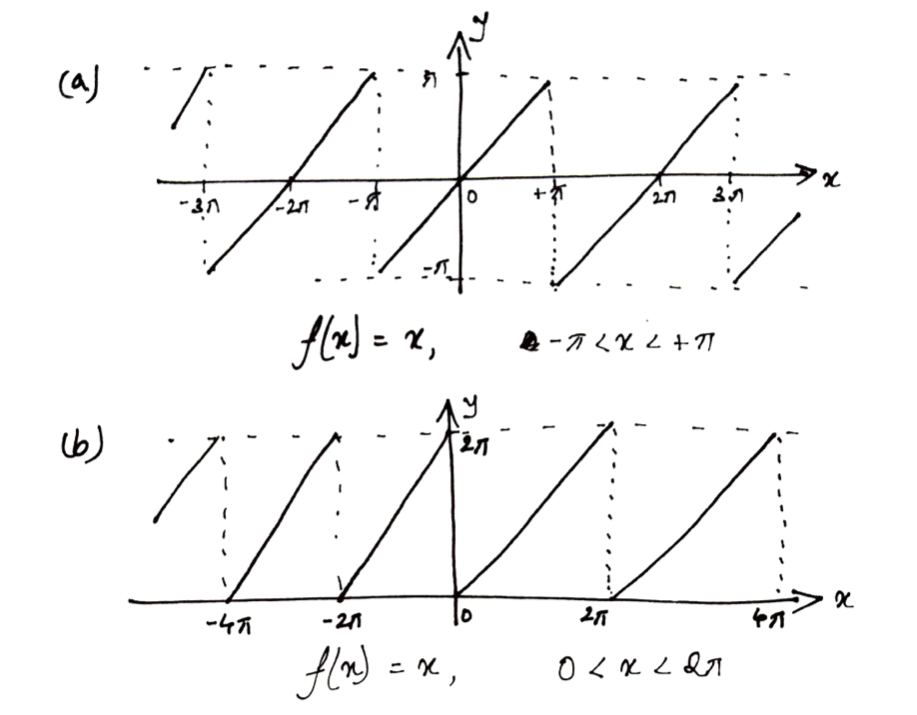
\includegraphics[scale=0.4]{./6_10.png}
        \end{center}

        \paragraph{Problem 14.} Sketch several periods of the following functions and expand them in a sine-cosine Fourier series and in a 
        complex exponential Fourier series.
        \begin{enumerate}
                \item \(f(x) = \sin{\pi x}, \quad -\frac{1}{2} < x < \frac{1}{2}\).
                \item \(f(x) = \sin{\pi x}, \quad 0 < x < 1\).
        \end{enumerate}
        \textit{Solution.}
        The functions $f$ have period $1$, so $\ell = 1 /2$.
        \begin{enumerate}
                \item We calculate 
                \[
                        c_0 = \int_{-1 /2}^{+1 /2} \sin{\pi x}\:dx = \frac{1}{\pi}\left[1 - 1\right] = 0.
                \]
                For $n \neq 0$, 
                \[
                        c_n = \int_{-1 /2}^{+1 /2} \sin{\pi x}\, e^{-2n\pi i x}\:dx 
                                = \frac{1}{2i} \int_{-1 /2}^{+1 /2}e^{(-2n + 1)\pi ix} - e^{(-2n - 1)\pi ix}\:dx
                \]
                \[
                        = \frac{1}{2\pi} \left[\frac{ie^{-n\pi i} + ie^{n\pi}}{2n - 1} - \frac{-ie^{-n\pi i} - ie^{n\pi i}}{2n + 1}\right]
                        = \frac{i}{2\pi}\cdot 2\cos{n\pi}\cdot\frac{4n}{4n^2 - 1}
                        = \frac{4ni(-1)^n}{\pi(4n^2 - 1)}.
                \]
                Thus, for $n > 0$, 
                \[
                        a_n = \frac{4ni(-1)^n - 4ni(-1)^{-n}}{\pi(4n^2 - 1)} = 0, \qquad
                        b_n = \frac{4ni^2(-1)^n + 4ni^2(-1)^{-n}}{\pi(4n^2 - 1)} = \frac{-8n(-1)^n}{\pi(4n^2 - 1)}.
                \]
                This means that
                \[
                        f(x) \;=\; \sum_{\substack{n = -\infty \\ n \neq 0}}^{+\infty} \frac{4ni}{\pi(4n^2 - 1)}(-1)^n e^{2n\pi ix} \;=\;
                                -\sum_{n = 1}^\infty \frac{8n}{\pi(4n^2 - 1)}(-1)^n\sin{2n\pi x}. \tag{$\star$}
                \]
                
                \item We calculate 
                \[
                        c_0 = \int_{0}^{1} \sin{\pi x}\:dx = \frac{1}{\pi}\left[-\cos{\pi} + 1\right] = \frac{2}{\pi}.
                \]
                For $n \neq 0$, 
                \[
                        c_n = \int_{0}^{1} \sin{\pi x}\, e^{-2n\pi i x}\:dx 
                                = \frac{1}{2i} \int_{0}^{1}e^{(-2n + 1)\pi ix} - e^{(-2n - 1)\pi ix}\:dx
                \]
                \[
                        = \frac{1}{2\pi} \left[\frac{-1 - 1}{2n - 1} - \frac{-1 - 1}{2n + 1}\right]
                        = \frac{1}{2\pi} \cdot (-2)\cdot\frac{2}{4n^2 - 1}
                        = \frac{-2}{\pi(4n^2 - 1)}.
                \]
                Thus, for $n > 0$, 
                \[
                        a_n = \frac{-2 - 2}{\pi(4n^2 - 1)} = \frac{-4}{\pi(4n^2 - 1)}, \qquad
                        b_n = \frac{-2i + 2i}{\pi(4n^2 - 1)} = 0.
                \]
                This means that
                \[
                        f(x) \;=\; \frac{2}{\pi} - \sum_{\substack{n = -\infty \\ n \neq 0}}^{+\infty} \frac{2}{\pi(4n^2 - 1)} e^{2n\pi ix} \;=\;
                                \frac{2}{\pi} - \sum_{n = 1}^\infty \frac{4}{\pi(4n^2 - 1)} \cos{2n\pi x}. \tag{$\star$}
                \]
        \end{enumerate}
        \begin{center}
                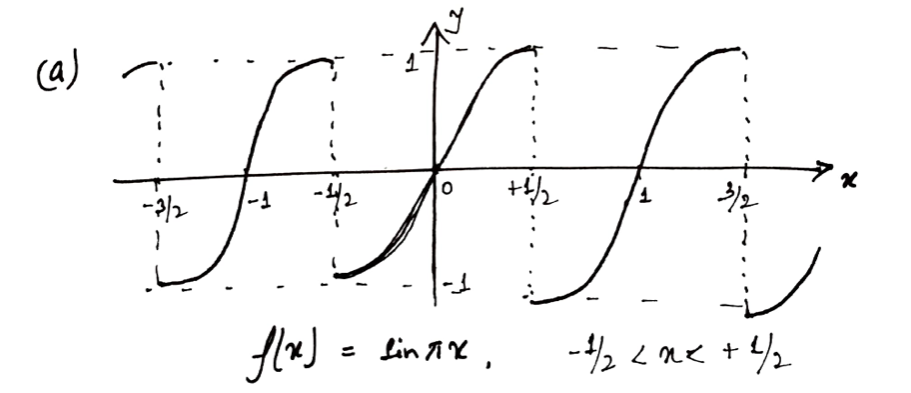
\includegraphics[scale=0.45]{./6_14a.png}
                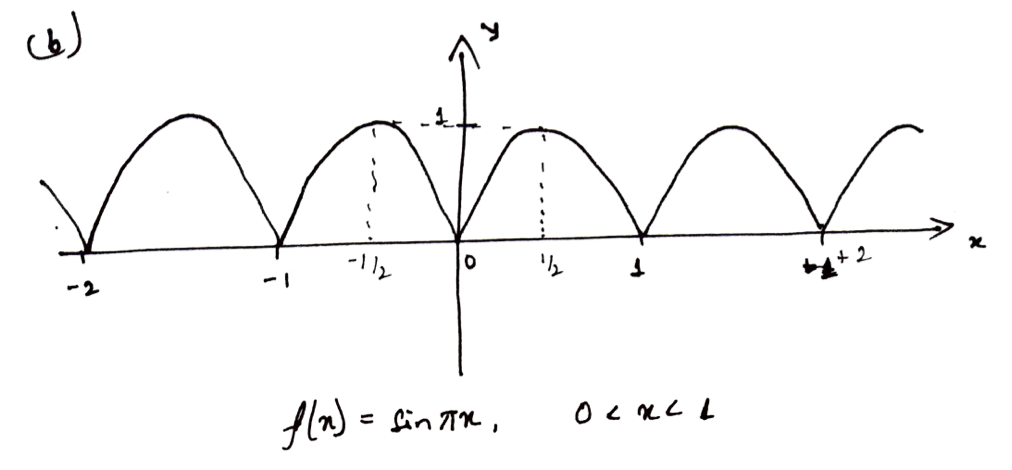
\includegraphics[scale=0.4]{./6_14b.png}
        \end{center}

        \paragraph{Problem 15} (c) Sketch (or computer plot) the following function on the interval $(−1, 1)$ and expand it in a 
        complex exponential series and in a sine-cosine series.
        \[
                f(x) = \begin{cases}
                        x + x^2, & -1 < x < 0, \\
                        x - x^2, & 0 < x < 1.
                \end{cases}
        \]
        \textit{Solution.} We calculate
        \[
                c_0 = \frac{1}{2}\int_{-1}^{+1} f(x)\:dx = \frac{1}{2}\int_0^1 f(x) + f(-x)\:dx = 0.
        \]
        For $n \neq 0$,
        \[
                c_n = \frac{1}{2}\int_{-1}^{+1} f(x)e^{-in\pi x}\:dx = \frac{1}{2}\int_0^1 (x - x^2)e^{-in\pi x} + (-x + x^2)e^{in\pi x}\:dx
        \]
        Now,
        \[
                \int_0^1 xe^{in\pi x}\:dx = \frac{1}{in\pi}xe^{in\pi x}\Big|_0^1 - \frac{1}{in\pi}\int_0^1 e^{in\pi x}\:dx
                        = \frac{1}{in\pi}e^{in\pi} + \frac{1}{n^2\pi^2}(e^{in\pi} - 1).
        \]
        \[
                \int_0^1 x^2e^{in\pi x}\:dx = \frac{1}{in\pi}x^2e^{in\pi x}\Big|_0^1 - \frac{2}{in\pi}\int_0^1 xe^{in\pi x}\:dx
                        = \frac{1}{in\pi}e^{in\pi} + \frac{2}{n^2\pi^2}e^{in\pi} - \frac{2}{in^3\pi^3}(e^{in\pi} - 1).
        \]
        Thus,
        \begin{align*}
                \int_0^1(-x + x^2)e^{in\pi x}\:dx &= \frac{1}{n^2\pi^2}( e^{in\pi}  + 1) - \frac{2}{in^3\pi^3}(e^{in\pi} - 1),\\
                \int_0^1(x - x^2)e^{-in\pi x}\:dx &= \frac{1}{n^2\pi^2}(-e^{-in\pi} - 1) - \frac{2}{in^3\pi^3}(e^{-in\pi} - 1).
        \end{align*}    
        Adding these together and halving,
        \[
                c_n = - \frac{2}{in^3\pi^3}(e^{in\pi} - 1).
        \]
        Note that this vanishes for even $n$. For odd $n$, we have $c_n = -4i /n^3\pi^3$. Thus, for odd $n > 1$,
        \[
                a_n = \cancel{-\frac{4i}{n^3\pi^3} + \frac{4i}{n^3\pi^3}} = 0, \qquad 
                b_n = -\frac{4i^2}{n^3\pi^3} - \frac{4i^2}{n^3\pi^3} = \frac{8}{n^3\pi^3}.
        \]
        Thus,
        \[
                f(x) \;=\; -\frac{4i}{\pi^3}\sum_{\substack{n = -\infty \\ \text{odd }n}}^{+\infty} \frac{1}{n^3} e^{n\pi ix} \;=\;
                        \frac{8}{\pi^3}\sum_{\substack{n = 1\\\text{odd }n}}^\infty \frac{1}{n^3} \sin{n\pi x}. \tag{$\star$}
        \]
        \begin{center}
                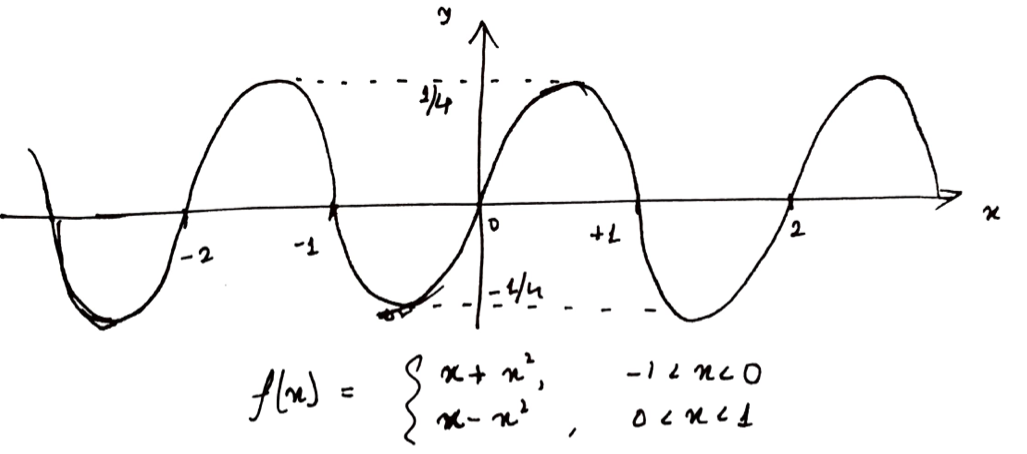
\includegraphics[scale=0.4]{./6_15.png}
        \end{center}
        
        \paragraph{Problem 17.} Sketch several periods of the following periodic function and expand it in a sine-cosine Fourier series and in a 
        complex exponential Fourier series.
        \[
                f(x) = \begin{cases}
                        0, & -1 < x < 0, \\
                        1, & 0 < x < 3.
                \end{cases}
        \]
        \textit{Solution.} The function $f$ has period $4$, so $\ell = 2$.
        We calculate
        \[
                c_0 = \frac{1}{4}\int_{-1}^3 f(x) \;dx = \frac{3}{4}.
        \]
        For $n \neq 0$, we have
        \[
                c_n = \frac{1}{4}\int_{-1}^3 f(x)e^{-in\pi x /2}\:dx = \frac{1}{4}\cdot \frac{-2}{in\pi}(e^{-3in\pi /2} - 1)
                        = -\frac{1}{2n\pi i} (e^{-3n\pi i /2} - 1).
        \]
        Thus, for $n > 1$, we have
        \begin{align*}
                a_n &= -\frac{(e^{-3n\pi i/2} - 1) - (e^{3n\pi i /2} - 1)}{2n\pi i} = \frac{1}{n\pi}\sin\frac{3n\pi}{2}, \\
                b_n &= -i\frac{(e^{-3n\pi i /2} - 1) + (e^{3n\pi i/2} - 1)}{2n\pi i} = -\frac{1}{n\pi}\cos\frac{3n\pi}{2} + \frac{1}{n\pi}.
        \end{align*}    
        Thus,
        \begin{align*}
                f(x) \;&=\; \frac{3}{4} \,-\, \sum_{\substack{n = -\infty \\ n \neq 0}}^{+\infty} \frac{1}{2n\pi i}(e^{-3n\pi i/2} - 1)e^{n\pi ix /2} \\
                        \;&=\; \frac{3}{4} \,+\, \sum_{n = 1}^\infty \frac{1}{n\pi}\sin\frac{3n\pi}{2}\cos\frac{n\pi x}{2} +
                                \frac{1}{n\pi}\left(1 - \cos\frac{3n\pi}{2}\right)\sin\frac{n\pi x}{2}. \tag{$\star$}
        \end{align*}
        \begin{center}
                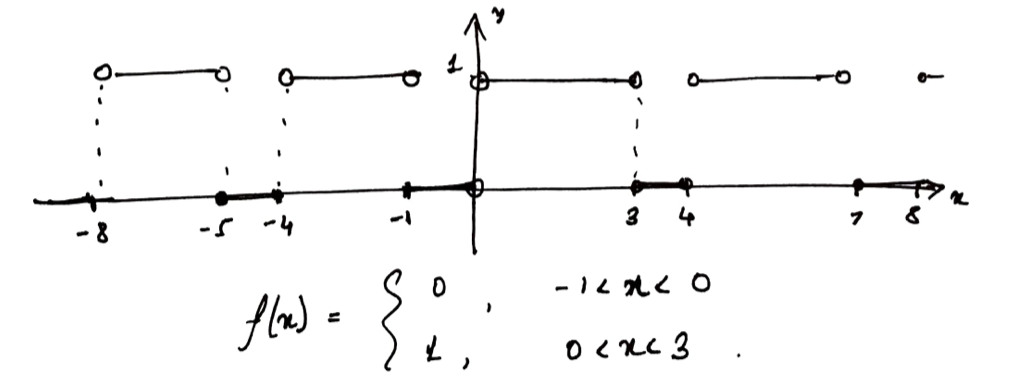
\includegraphics[scale=0.4]{./6_17.png}
        \end{center}
        
        \paragraph{Problem 20.} Sketch several periods of the following periodic function and expand it in a sine-cosine Fourier series and in a 
        complex exponential Fourier series.
        \[
                f(x) = \begin{cases}
                        x/2, & 0 < x < 2, \\
                        1, & 2 < x < 3.
                \end{cases}
        \]
        \textit{Solution.} The function $f$ has period $3$, so $\ell = 3 /2$.
        We calculate
        \[
                c_0 = \frac{1}{3}\int_0^3 f(x)\:dx = \frac{1}{3}\cdot\frac{x^2}{4}\Bigg|_0^2 + \frac{1}{3} = \frac{2}{3}.
        \]
        For $n\neq 0$, we have
        \begin{align*}
        c_n &= \frac{1}{3}\int_0^2 \frac{x}{2}e^{-2in\pi x/3}\:dx + \frac{1}{3}\int_2^3 e^{-2in\pi x/3}\:dx \\
                &= -\frac{1}{4n\pi i}xe^{-2in\pi x/3}\Big|_0^2 + \frac{1}{4n\pi i}\int_0^2 e^{-2in\pi x/3}\:dx - 
                        \frac{1}{2n\pi i}e^{-2in\pi x/3}\Big|_2^3 \\
                &= -\frac{1}{2n\pi i}\cancel{e^{-4in\pi/3}} + \frac{3}{8n^2\pi^2}(e^{-4in\pi/3} - 1) - \frac{1}{2n\pi i}(1 - \cancel{e^{-4n\pi i/3}}) \\
                &= -\frac{1}{2n\pi i} - \frac{3}{8n^2\pi^2} + \frac{3}{8n^2\pi^2}e^{-4in\pi/3}. 
        \end{align*}
        Thus, for $n > 1$,
        \begin{align*}
                a_n &= \cancel{-\frac{1}{2n\pi i} + \frac{1}{2n\pi i}} - \frac{3}{8n^2\pi^2} - \frac{3}{8n^2\pi^2} + \frac{3}{8n^2\pi^2}e^{-4in\pi/3} 
                        + \frac{3}{8n^2\pi^2}e^{4in\pi/3} \\
                        &= \frac{3}{4n^2\pi^2}\left(\cos\frac{4n\pi}{3} - 1\right), \\
                b_n &= -\frac{1}{2n\pi} - \frac{1}{2n\pi} - \cancel{\frac{3i}{8n^2\pi^2} + \frac{3i}{8n^2\pi^2}} + \frac{3i}{8n^2\pi^2}e^{-4in\pi/3}
                        - \frac{3i}{8n^2\pi^2}e^{4in\pi/3} \\
                        &= -\frac{1}{n\pi} + \frac{3}{4n^2\pi^2}\sin\frac{4n\pi}{3}.
        \end{align*}
        We can separate these into 3 cases, based on the residue of $n$ modulo $3$.
        Note that $\cos(4(3k)\pi /3) = \sin(4(3k)\pi /3) = 0$, $\cos(4(3k \pm 1)\pi /3) = -1 /2$, and $\sin(4(3k \pm 1)\pi /3) = \mp \sqrt{3}/{2}$.
        Thus,
        \begin{center}
        \begin{tabular}{c||c|c|c}
                $n \bmod 3$     & 0                     & 1                             & 2 \\ \hline\hline
                $a_n$           & 0                     & $-\displaystyle\frac{9}{8n^2\pi^2}$          & $-\displaystyle\frac{9}{8n^2\pi^2}$ \\
                $b_n$           & $-\displaystyle\frac{1}{n\pi}$       & $-\displaystyle\frac{1}{n\pi} - \displaystyle\frac{3\sqrt{3}}{8n^2\pi^2}$ & 
                                                                $-\displaystyle\frac{1}{n\pi} + \displaystyle\frac{3\sqrt{3}}{8n^2\pi^2}$
        \end{tabular}
        \end{center}
        We thus expand
        \begin{align*}
                f(x) \;&=\; \frac{2}{3} \,+\, \sum_{\substack{n = -\infty \\ n \neq 0}}^{+\infty} \left(-\frac{1}{2n\pi i} - 
                                \frac{3}{8n^2\pi^2} + \frac{3}{8n^2\pi^2}e^{-4in\pi/3}\right)e^{2in\pi x/3} \\
                        \;&=\; \frac{2}{3} \,+\, \sum_{n = 1}^\infty \frac{3}{4n^2\pi^2}\left(\cos\frac{4n\pi}{3} - 1\right)\cos\frac{2n\pi x}{3} +
                                \left(-\frac{1}{n\pi} + \frac{3}{4n^2\pi^2}\sin\frac{4n\pi}{3}\right)\sin\frac{2n\pi x}{3}. \tag{$\star$}
        \end{align*}
        \begin{center}
                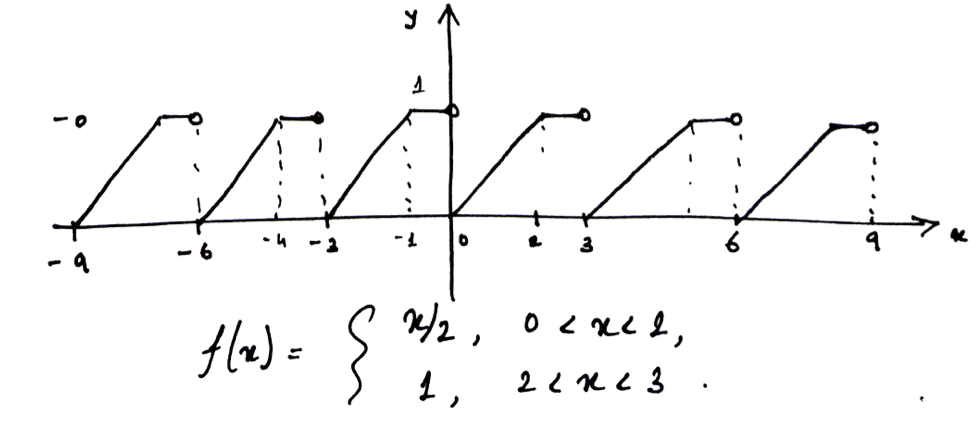
\includegraphics[scale=0.4]{./6_20.png}
        \end{center}

\end{document}
